%--------------------------------------------------
%    PACKAGES AND THEMES
%------------------------------------
\documentclass[aspectratio=169,xcolor=dvipsnames]{beamer}
\makeatletter
\def\input@path{{theme/}}
\makeatother
\usetheme{SimplePlus}
\usepackage{hyperref}
\usepackage{graphicx}
\usepackage{booktabs}
\usepackage{natbib}
\usepackage{amsmath,amssymb}
\usepackage{bm}
\usepackage{tikz}
\usetikzlibrary{arrows.meta, positioning, shapes.geometric}

% Para placeholder de figuras
\newcommand{\placeholder}[2][0.8\textwidth]{%
    \begin{center}
    \fcolorbox{gray}{gray!10}{%
        \parbox{#1}{\centering\vspace{1cm}\textit{#2}\vspace{1cm}}%
    }
    \end{center}
}

%----------------------------------------------------------------------------------------
%    TITLE PAGE
%----------------------------------------------------------------------------------------
\title{Reducción de Rizo de Par en Motores BLDC mediante\\MPC con Estimación Adaptable de BEMF}
\subtitle{FCS-M2PC + ADALINE}
\author{Alejandro León}
\institute
{
    Instituto de Ingeniería \\
    Universidad Nacional Autónoma de México
}
\date{\today}

%----------------------------------------------------------------------------------------
%    PRESENTATION SLIDES
%----------------------------------------------------------------------------------------
\begin{document}

\begin{frame}
    \titlepage
\end{frame}

\begin{frame}{Contenido}
    \tableofcontents
\end{frame}

%----------------- section 1 --------------------
\section{Introducción y Planteamiento}
\input{sections/01_introduction.tex}

%----------------- section 2 --------------------
\section{Marco Teórico: FCS-M2PC}
% ==============================================================
% SECCIÓN 2: MARCO TEÓRICO — FCS-M2PC
% ==============================================================

% --- Slide 5: Modelo del motor ---
\begin{frame}{Modelo del Motor BLDC en $\alpha\beta$}
    Dinámica eléctrica en el marco estacionario de Clarke:
    \begin{equation}
        \frac{d}{dt}\begin{bmatrix} i_\alpha \\ i_\beta \end{bmatrix} 
        = \frac{1}{L}\left(
            \begin{bmatrix} u_\alpha \\ u_\beta \end{bmatrix}
            - R \begin{bmatrix} i_\alpha \\ i_\beta \end{bmatrix}
            - \begin{bmatrix} e_\alpha(\theta_e) \\ e_\beta(\theta_e) \end{bmatrix}
        \right)
    \end{equation}
    
    donde la BEMF depende de la forma de onda \textbf{shape} $\mathbf{s}(\theta_e)$:
    \begin{equation}
        \mathbf{e}_{\alpha\beta}(\theta_e) = K_e \cdot \omega_m \cdot \mathbf{s}(\theta_e)
    \end{equation}
    
    \begin{itemize}
        \item Si $\mathbf{s}(\theta_e) = [\sin\theta_e,\; -\cos\theta_e]^T$ $\rightarrow$ motor senoidal ideal
        \item Motor real: $\mathbf{s}(\theta_e)$ contiene armónicos 5to, 7mo, 11vo...
        \item \textbf{El conocimiento preciso de $\mathbf{s}(\theta_e)$ es clave} para generar referencias de corriente que produzcan torque constante.
    \end{itemize}
\end{frame}

% --- Slide 6: FCS-M2PC ---
\begin{frame}{FCS-M2PC: Control Predictivo con Dos Vectores por Período}
    \textbf{Idea clave} (Coronado-Andrade et al., 2025): dividir $T_s$ en sub-intervalos y aplicar \textbf{combinaciones} de dos vectores activos + vector nulo.
    
    \vspace{0.2cm}
    
    \begin{columns}[T]
    \begin{column}{0.55\textwidth}
        Predicción de corriente al fin del período:
        \begin{equation}
            \mathbf{i}(k{+}1) = \mathbf{i}(k) + \mathbf{f}_1 t_1 + \mathbf{f}_2 t_2 + \mathbf{f}_0 t_0
        \end{equation}
        donde $\mathbf{f}_j = \frac{1}{L}(\mathbf{u}_j - \mathbf{e} - R\mathbf{i})$ y $t_1+t_2+t_0 = T_s$.
        
        \vspace{0.3cm}
        
        Función de costo:
        \begin{equation}
            g^* = \min_{t_1, t_2} \left\| \mathbf{i}^*_{\text{ref}}(k{+}1) - \mathbf{i}_{\text{pred}}(k{+}1) \right\|^2
        \end{equation}
        
        \vspace{0.2cm}
        \textbf{Ventaja vs.\ FCS-MPC clásico:} reducción de 75--80\% en RMSE de corriente \citep{coronado2025}.
    \end{column}
    \begin{column}{0.42\textwidth}
    \centering
    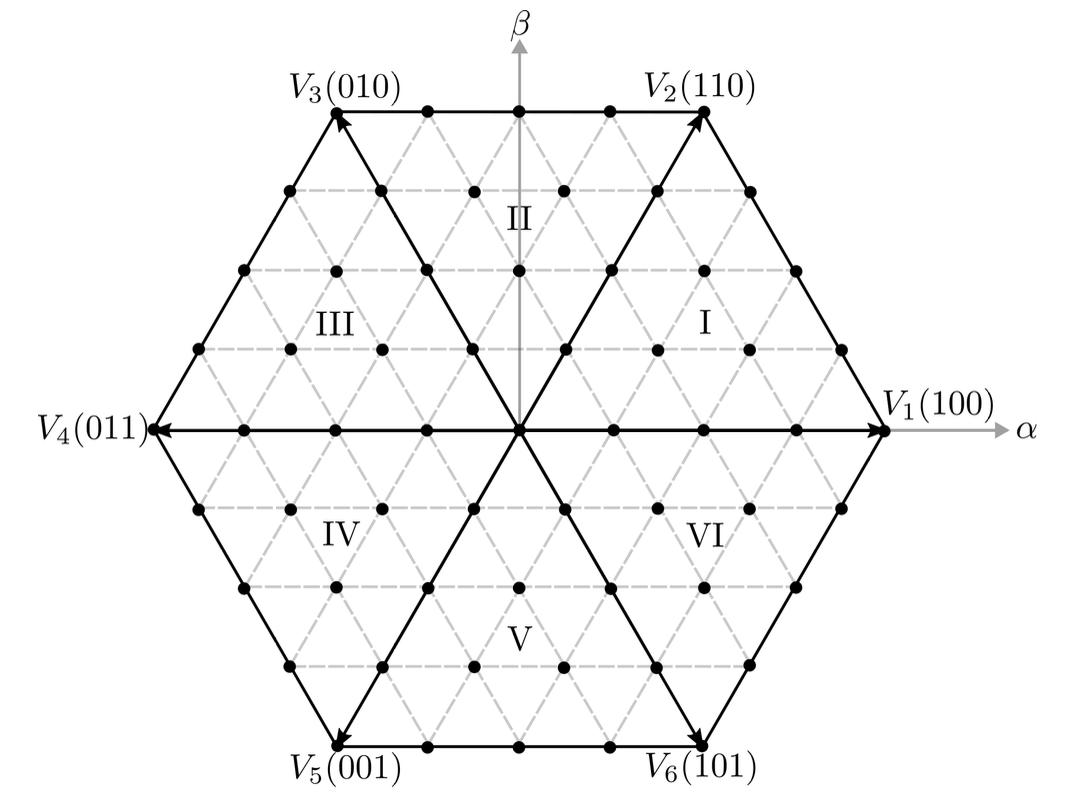
\includegraphics[width=0.95\linewidth]{fig/m2pc_vector_diagram.png}
    {\footnotesize Diagrama vectores de voltaje}
    \end{column}
    \end{columns}
\end{frame}

% --- Slide 7: El rol de la BEMF en el M2PC ---
\begin{frame}{¿Por Qué la BEMF Importa Tanto en el M2PC?}
    La BEMF aparece en \textbf{dos lugares críticos}:
    
    \vspace{0.3cm}
    
    \begin{columns}[T]
    \begin{column}{0.48\textwidth}
        \begin{block}{1. Generación de $\mathbf{i}^*_{\text{ref}}$}
            Para torque constante $T_{\text{ref}}$:
            \begin{equation}
                \mathbf{i}^* = \frac{T_{\text{ref}}}{K_t \|\mathbf{s}\|^2} \cdot \mathbf{s}(\theta_e)
            \end{equation}
            Si $\mathbf{s}$ es incorrecto $\rightarrow$ la referencia tiene armónicos $\rightarrow$ torque oscila.
        \end{block}
    \end{column}
    \begin{column}{0.48\textwidth}
        \begin{block}{2. Modelo de predicción}
            \begin{equation}
                \mathbf{i}_{\text{pred}} = \mathbf{i} + \frac{T_s}{L}(\mathbf{u} - \hat{\mathbf{e}} - R\mathbf{i})
            \end{equation}
            Si $\hat{\mathbf{e}} \neq \mathbf{e}_{\text{real}}$ $\rightarrow$ predicción sesgada $\rightarrow$ vector de voltaje subóptimo.
        \end{block}
    \end{column}
    \end{columns}
    
    \vspace{0.5cm}
    
    \begin{center}
        \fcolorbox{red}{red!5}{\parbox{0.85\textwidth}{\centering
            \textbf{Conclusión:} Un modelo preciso de $\mathbf{s}(\theta_e)$ mejora \textit{simultáneamente} la referencia y la predicción.\\
            $\rightarrow$ Motivación para aprender $\mathbf{s}(\theta_e)$ del motor real.
        }}
    \end{center}
\end{frame}

%----------------- section 3 --------------------
\section{ADALINE: Aprendizaje de BEMF}
% ==============================================================
% SECCIÓN 3: ADALINE — APRENDIZAJE DE BEMF
% ==============================================================

% --- Slide 8: ¿Qué es ADALINE? ---
\begin{frame}{ADALINE: Adaptive Linear Neuron (Widrow-Hoff, 1960)}
    Red neuronal de \textbf{una sola capa, sin no-linealidad}, con base de entrada de Fourier:
    
    \begin{equation}
        \hat{s}_\alpha(\theta) = \mathbf{w}_\alpha^T \mathbf{x}(\theta) = \sum_{n=1}^{H} \left[ w_n^c \cos(n\theta) + w_n^s \sin(n\theta) \right]
    \end{equation}
    
    donde el vector de regresores es:
    \begin{equation}
        \mathbf{x}(\theta) = \begin{bmatrix} \cos\theta & \sin\theta & \cos 2\theta & \sin 2\theta & \cdots & \cos H\theta & \sin H\theta \end{bmatrix}^T \in \mathbb{R}^{2H}
    \end{equation}
    
    \begin{itemize}
        \item Con $H = 10$ armónicos: \textbf{40 parámetros totales} (20 por eje $\alpha, \beta$).
        \item Los pesos $w_n^c, w_n^s$ \textbf{son los coeficientes de Fourier} de la BEMF.
        \item Interpretación física directa: $|w_5| = $ amplitud del 5to armónico.
    \end{itemize}
\end{frame}

% --- Slide 9: ¿Por qué ADALINE y no una NN profunda? ---
\begin{frame}{¿Por Qué ADALINE y No una Red Neuronal Profunda?}
    \begin{columns}[T]
    \begin{column}{0.48\textwidth}
        \begin{block}{Red Profunda (BEMFNet)}
            \begin{itemize}
                \item 4 capas ocultas (64--128 neuronas)
                \item $\sim$25,000 parámetros
                \item Entrenamiento: 300 epochs, $\sim$30 s
                \item Backpropagation: $O(N_{\text{params}})$ por paso
                \item Mínimo local (no convexo)
                \item Pesos: caja negra
            \end{itemize}
        \end{block}
    \end{column}
    \begin{column}{0.48\textwidth}
        \begin{exampleblock}{ADALINE + Fourier}
            \begin{itemize}
                \item 1 capa, sin activación
                \item \textbf{40 parámetros}
                \item Entrenamiento: pseudoinversa, $\sim$12 ms
                \item LMS online: $O(2H)$ por paso
                \item \textbf{Óptimo global} (problema convexo)
                \item Pesos = espectro de Fourier
            \end{itemize}
        \end{exampleblock}
    \end{column}
    \end{columns}
    
    \vspace{0.4cm}
    
    \begin{center}
        \fcolorbox{ForestGreen}{green!5}{\parbox{0.85\textwidth}{\centering
            La BEMF es una \textbf{función periódica de $\theta$} $\rightarrow$ la serie de Fourier es su representación \textbf{natural y óptima}.\\
            Usar una NN profunda para esto es \textit{usar un aproximador universal cuando existe la solución exacta}.
        }}
    \end{center}
\end{frame}

% --- Slide 10: Entrenamiento offline ---
\begin{frame}{Fase 0: Entrenamiento Offline (Pseudoinversa)}
    Dado el dataset $\{(\theta_k, s_{\alpha,k}, s_{\beta,k})\}_{k=1}^{N}$, construimos:
    \begin{equation}
        \mathbf{X} = \begin{bmatrix} \mathbf{x}(\theta_1)^T \\ \vdots \\ \mathbf{x}(\theta_N)^T \end{bmatrix} \in \mathbb{R}^{N \times 2H}, \qquad
        \mathbf{W}^* = (\mathbf{X}^T\mathbf{X})^{-1}\mathbf{X}^T \mathbf{S} = \mathbf{X}^\dagger \mathbf{S}
    \end{equation}
    
    \begin{columns}[T]
    \begin{column}{0.42\textwidth}
        \centering
        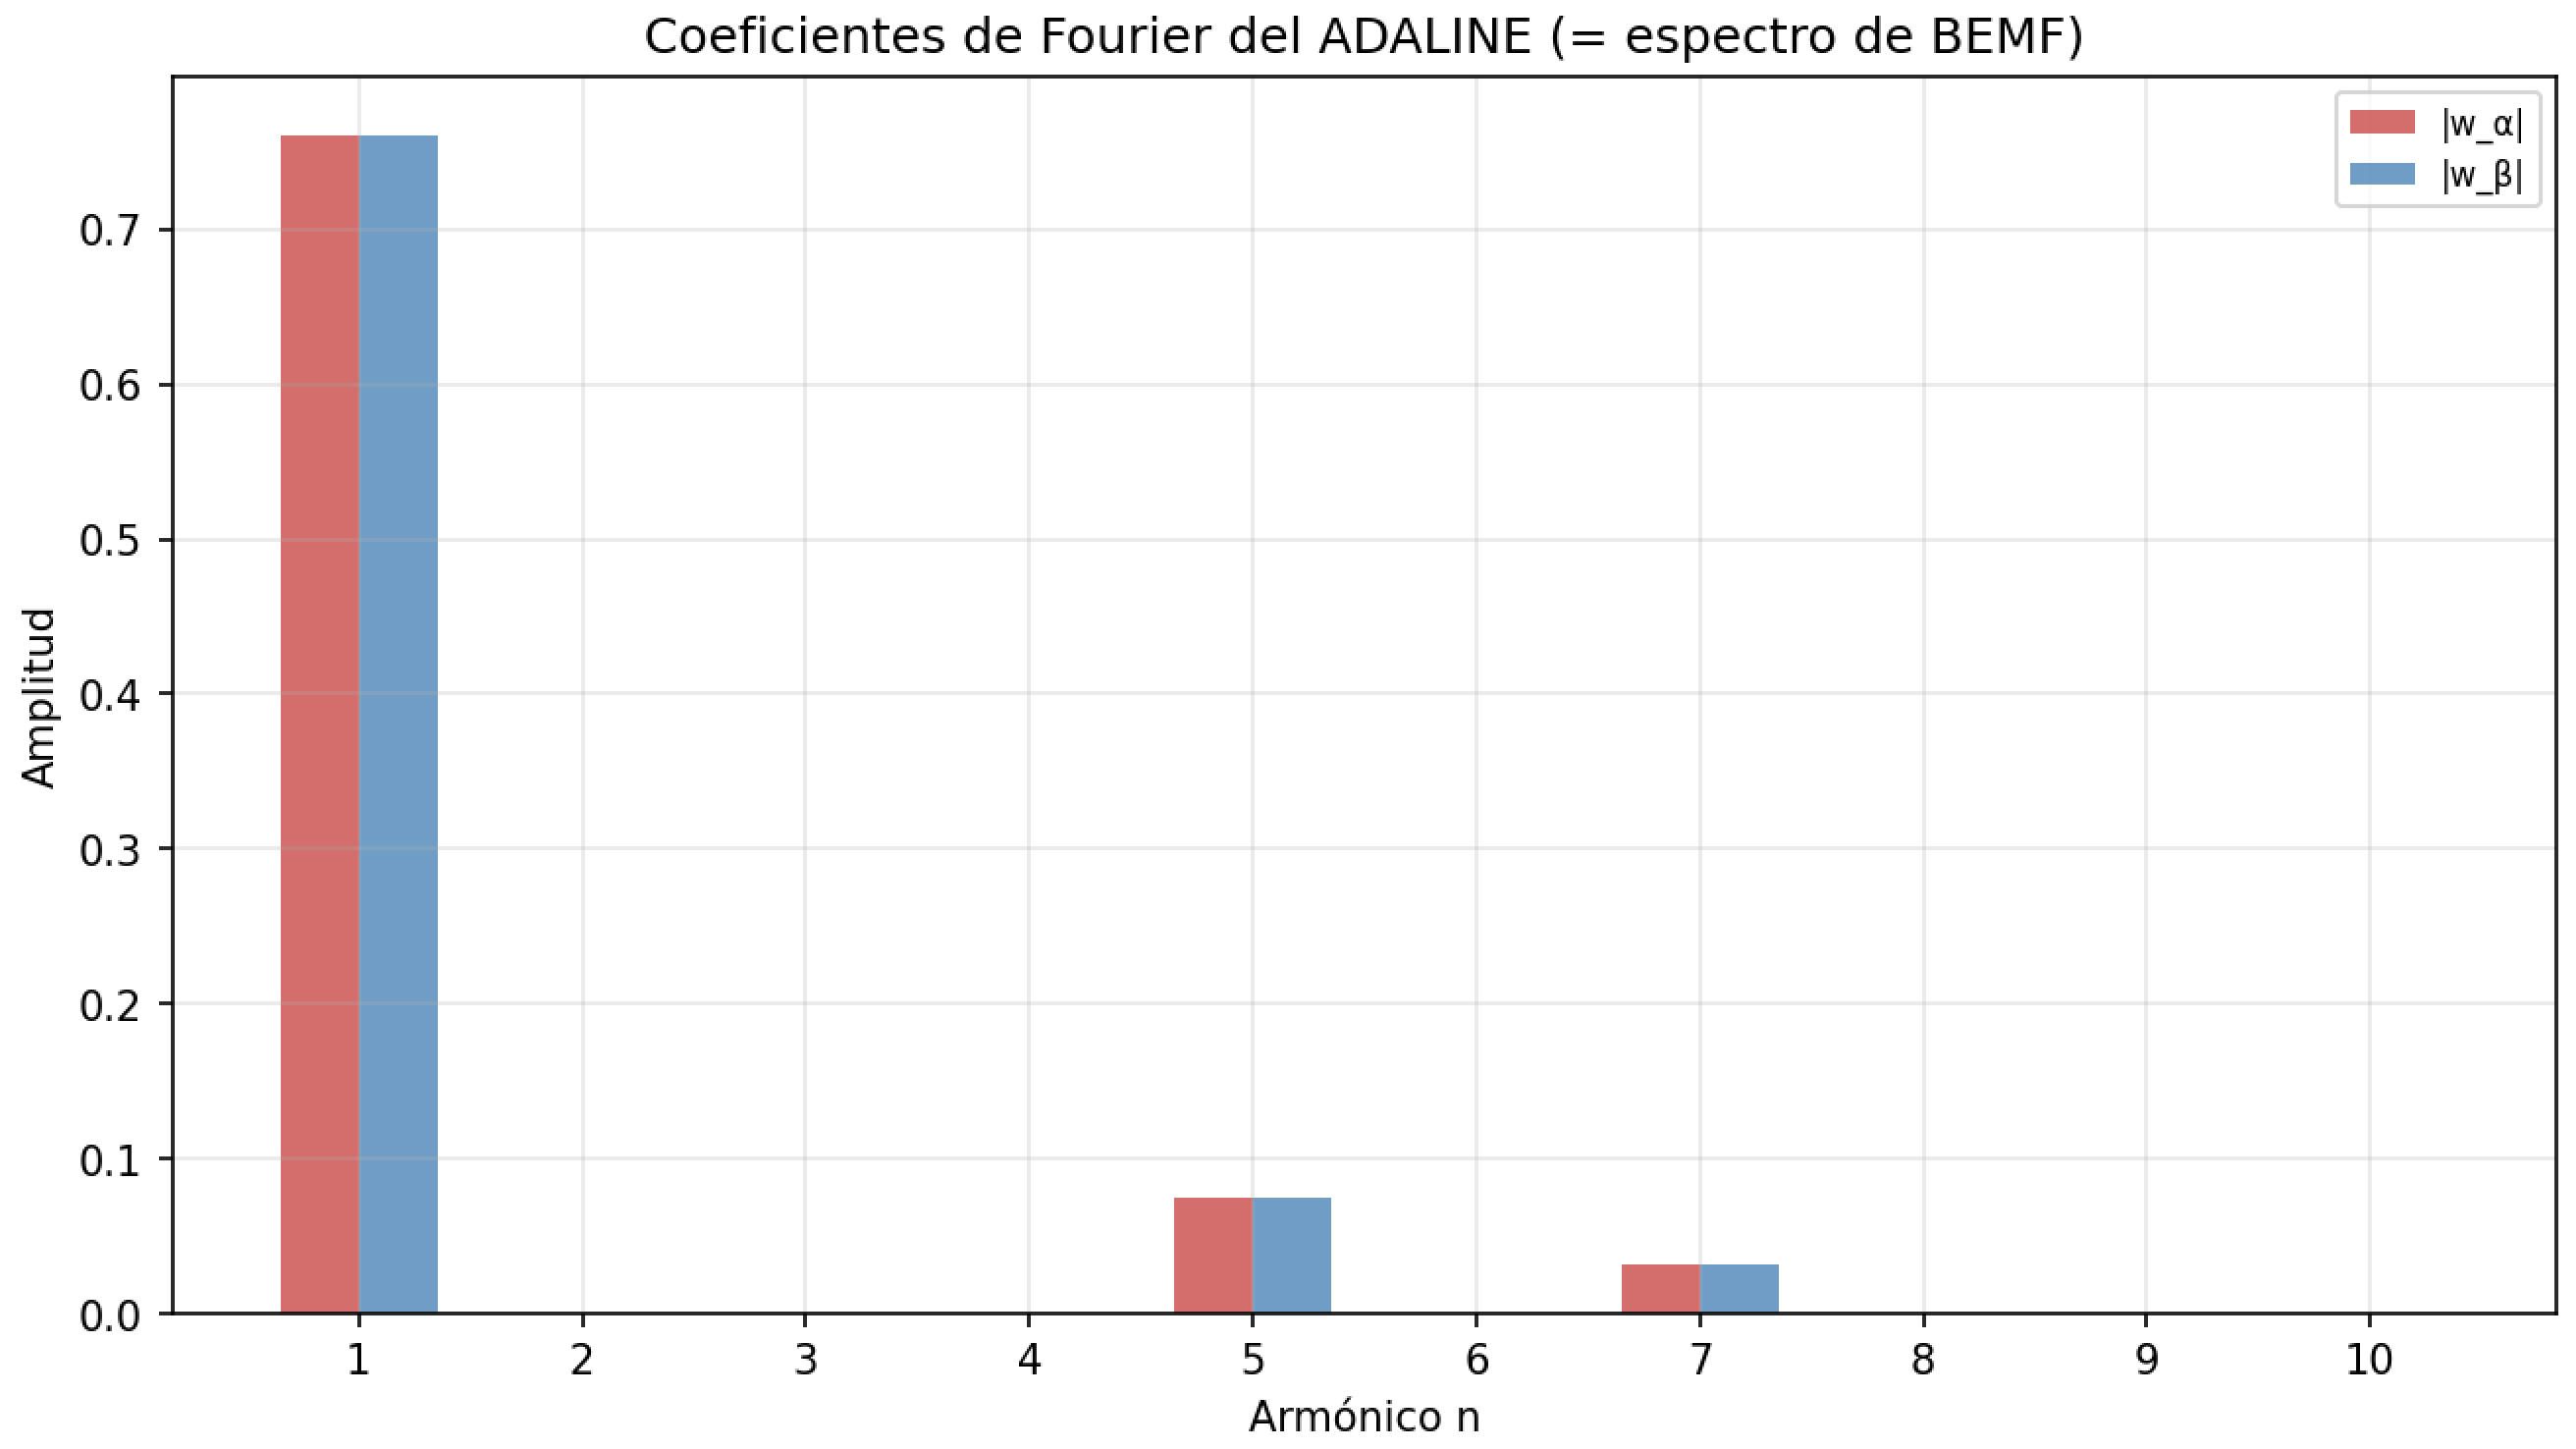
\includegraphics[width=0.99\linewidth]{fig/adaline_fourier_coeffs.png}
        {\footnotesize Coeficientes de fourier por armónico}
    \end{column}
    \begin{column}{0.42\textwidth}
        \centering
        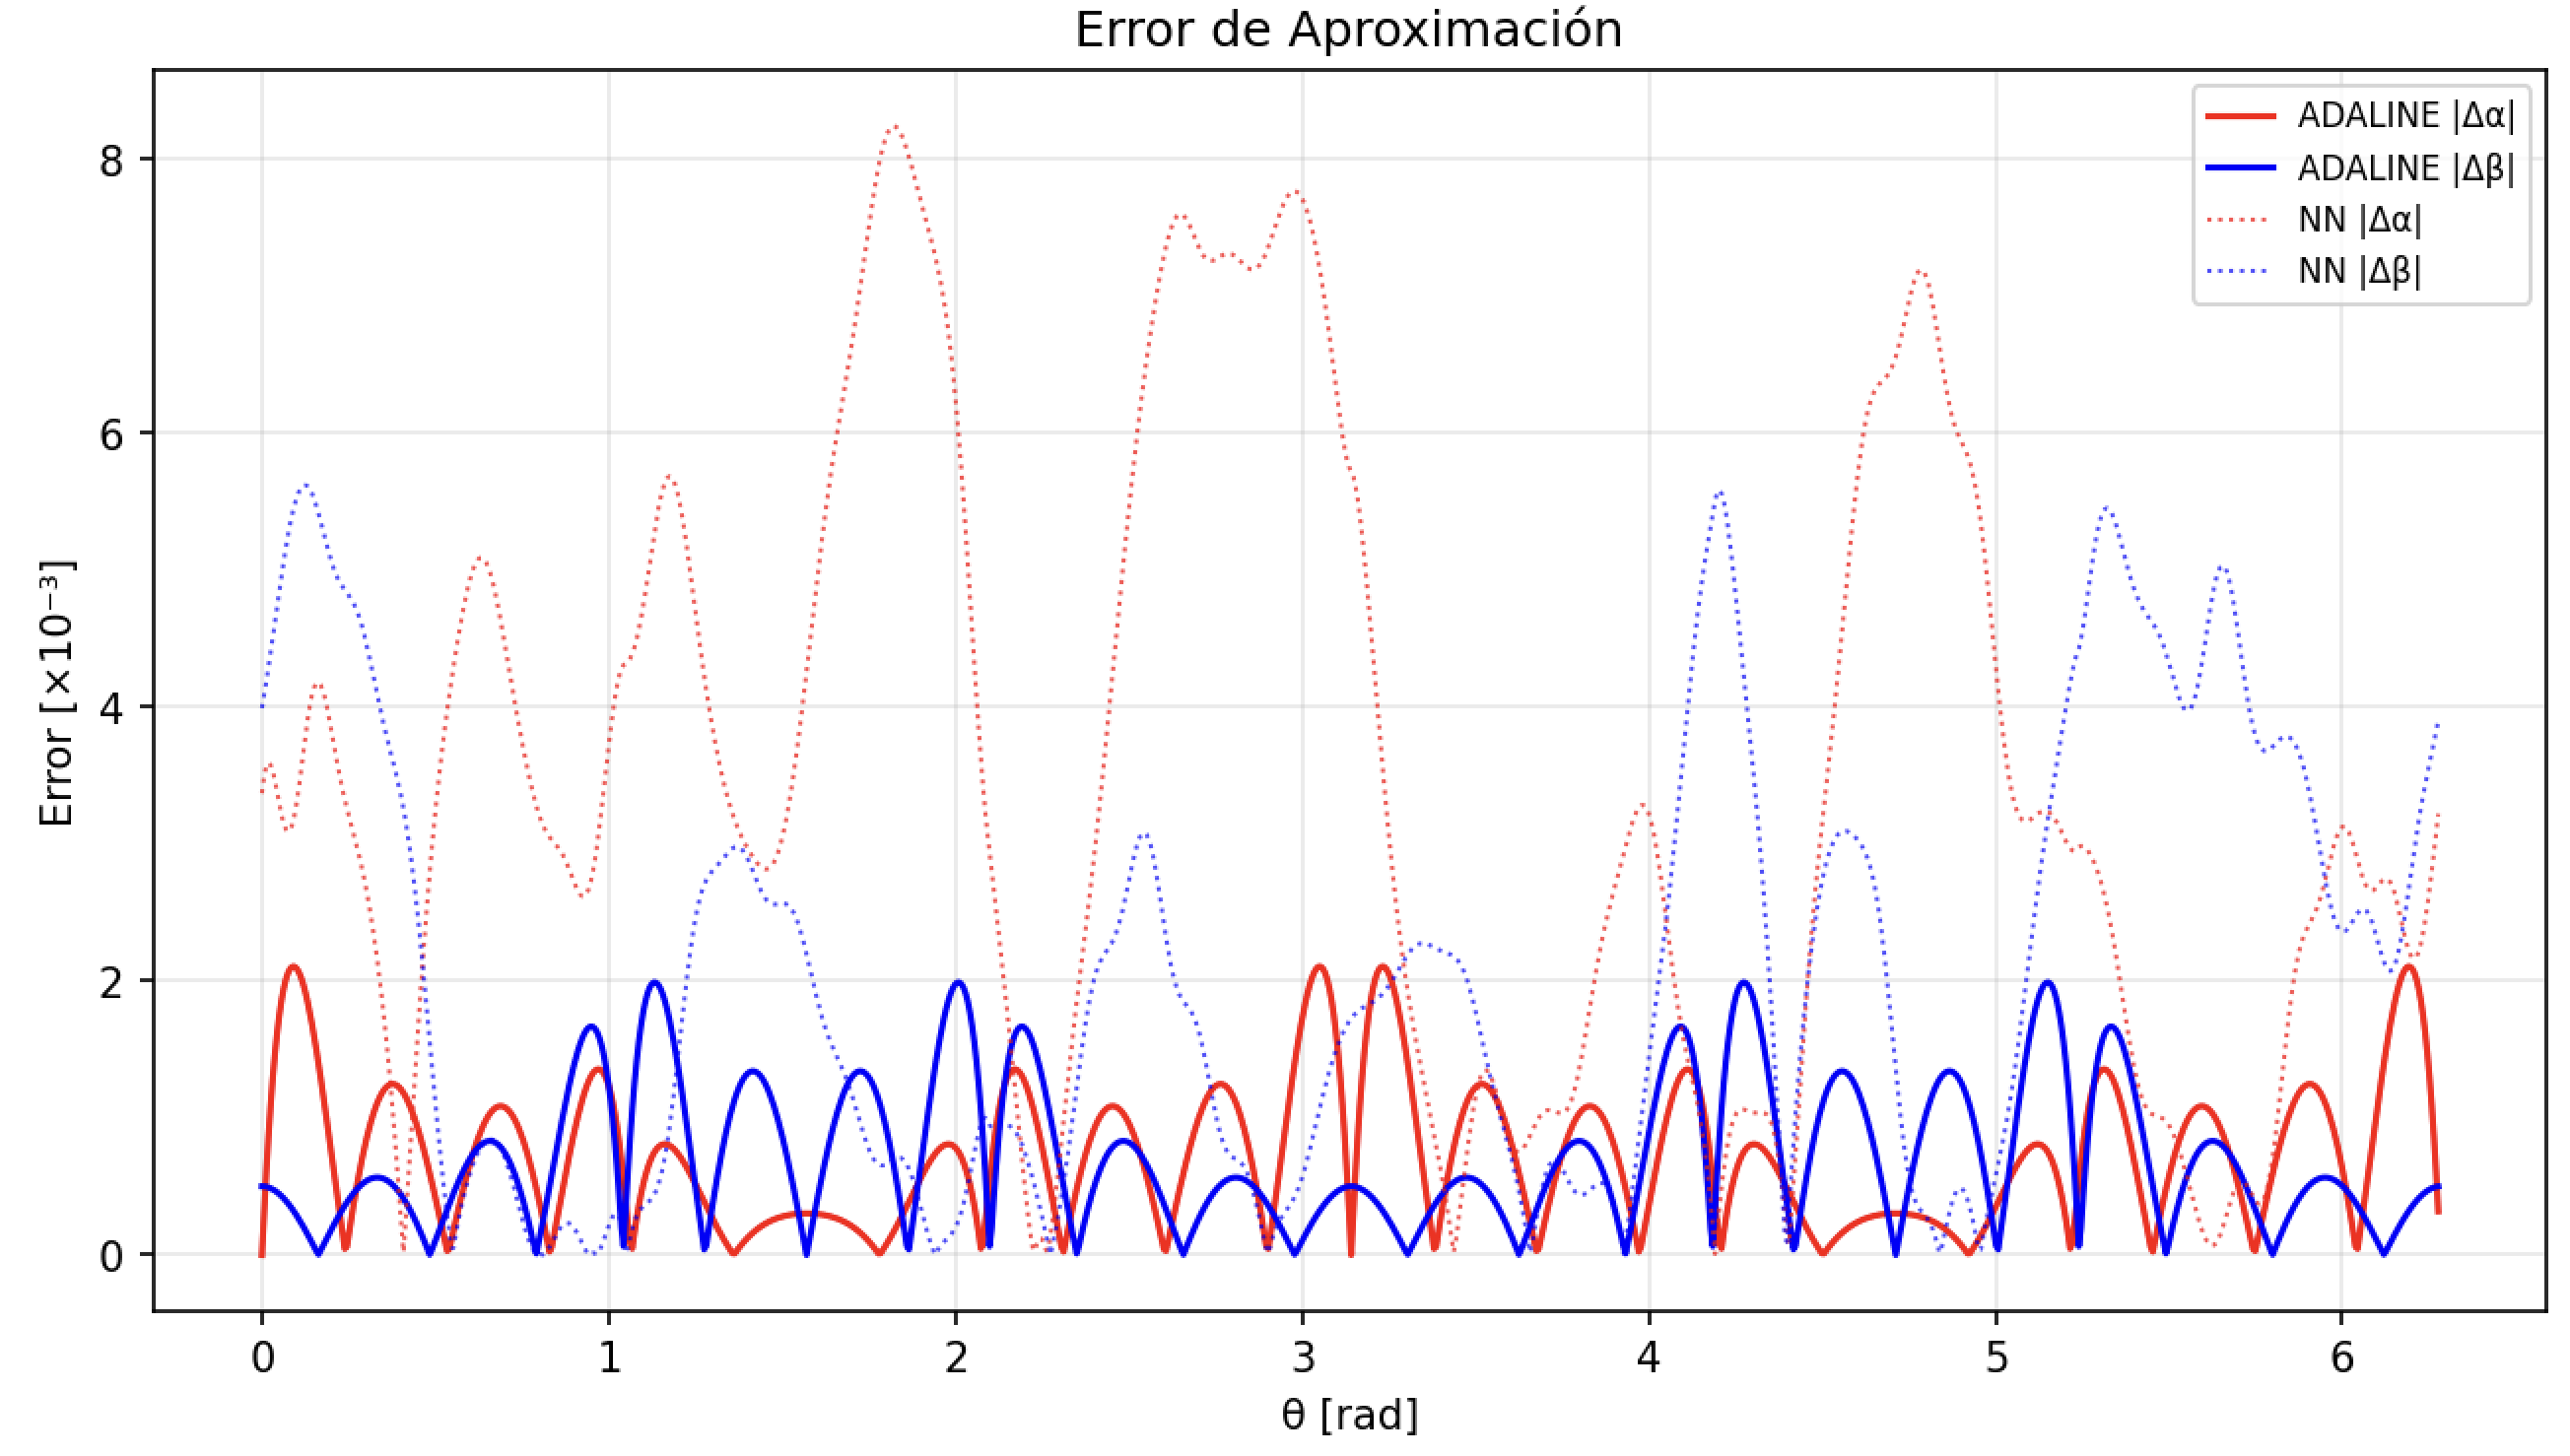
\includegraphics[width=0.99\linewidth]{fig/adaline_vs_nn_alpha.png}
        {\footnotesize ADALINE vs NN}
    \end{column}
    \end{columns}
\end{frame}

% --- Slide 11: ADALINE online con LMS ---
\begin{frame}{Fase 1: Aprendizaje Online con LMS}
    \textbf{Ley de actualización} (Least Mean Squares):
    \begin{equation}
        \mathbf{w}(k+1) = \mathbf{w}(k) + \mu \cdot \underbrace{\left[s_{\text{obs}}(k) - \mathbf{w}^T(k)\mathbf{x}(\theta_k)\right]}_{\text{error de estimación } \epsilon(k)} \cdot \mathbf{x}(\theta_k)
    \end{equation}
    
    \vspace{0.2cm}
    
    \begin{columns}[T]
    \begin{column}{0.48\textwidth}
        \textbf{Propiedades clave:}
        \begin{itemize}
            \item \textbf{Convergencia:} $0 < \mu < 4$ (base ortogonal $\rightarrow$ $\lambda_{\max} = 1/2$)
            \item \textbf{Velocidad:} $\tau \approx 1/\mu$ pasos $\approx$ 1--2 rev eléctricas
            \item \textbf{Misadjustment:} $M \approx \mu H$ (residuo en régimen permanente)
            \item \textbf{Costo:} 1 producto punto por paso ($\sim$\textbf{microsegundos} en DSP)
        \end{itemize}
    \end{column}
    \begin{column}{0.48\textwidth}
        \textbf{¿Qué significa esto?}
        \begin{itemize}
            \item El motor se \textbf{auto-calibra} en $\sim$50 ms
            \item No necesita datos previos del fabricante
            \item Se adapta a cambios térmicos, envejecimiento, tolerancias de fabricación
            \item \textbf{Implementable en DSP} (TMS320F28xxx) sin modificaciones de hardware
        \end{itemize}
    \end{column}
    \end{columns}
\end{frame}

% --- Slide 12: Idoneidad del ADALINE ---
\begin{frame}{¿Por Qué ADALINE es \textit{Idóneo} para Este Problema?}
    
    Tres razones estructurales (no cosméticas):
    
    \vspace{0.3cm}
    
    \begin{enumerate}
        \item \textbf{La BEMF es periódica en $\theta$} $\rightarrow$ la serie de Fourier es completa y ortogonal para funciones periódicas. No hay pérdida de generalidad al truncar a $H$ armónicos si la energía espectral por encima de $H$ es despreciable.
        
        \vspace{0.2cm}
        
        \item \textbf{La base $\{\cos n\theta, \sin n\theta\}$ tiene $\|\mathbf{x}\|^2 = H$ constante} $\rightarrow$ todos los modos convergen a la misma velocidad (no hay \textit{eigenvalue spread}). El LMS es \textbf{óptimamente condicionado} para esta base.
        
        \vspace{0.2cm}
        
        \item \textbf{Los pesos son directamente los coeficientes de Fourier} $\rightarrow$ se puede inspeccionar \textit{qué armónicos tiene el motor} mirando $|w_n|$. Además, estos pesos son la \textbf{inicialización natural} para un controlador repetitivo que necesita conocer el espectro del disturbio.
    \end{enumerate}
    
    \vspace{0.3cm}
    
    \begin{center}
        \small
        $\underbrace{\text{ADALINE offline}}_{\text{Fase 0: modelo base}}
        \;\xrightarrow{\text{LMS}}\;
        \underbrace{\text{ADALINE online}}_{\text{Fase 1: auto-calibración}}
        \;\xrightarrow{\text{pesos} \rightarrow \text{espectro}}\;
        \underbrace{\text{Control Repetitivo}}_{\text{Fase 3: rechazo periódico}}$
    \end{center}
\end{frame}

%----------------- section 4 --------------------
\section{Resultados de Simulación}
% ==============================================================
% SECCIÓN 4: RESULTADOS DE SIMULACIÓN
% ==============================================================

% --- Slide 13: Setup de simulación ---
\begin{frame}{Configuración de Simulación}
    \begin{columns}[T]
    \begin{column}{0.48\textwidth}
        \begin{table}[h]
        \centering
        \small
        \begin{tabular}{@{}ll@{}}
        \toprule
        \textbf{Parámetro} & \textbf{Valor} \\
        \midrule
        Motor & BLY-344S-240V \\
        $R$ & 1.2 $\Omega$ \\
        $L$ & 2.05 mH \\
        $K_e$ & 0.404 V$\cdot$s/rad \\
        $K_t$ & 0.660 Nm/A \\
        Polos & 4 \\
        $J$ & $2.79 \times 10^{-4}$ kg$\cdot$m$^2$ \\
        $V_{DC}$ & 240 V \\
        \bottomrule
        \end{tabular}
        \end{table}
    \end{column}
    \begin{column}{0.48\textwidth}
        \begin{table}[h]
        \centering
        \small
        \begin{tabular}{@{}ll@{}}
        \toprule
        \textbf{Control} & \textbf{Valor} \\
        \midrule
        $T_s$ & 50 $\mu$s (20 kHz) \\
        $\rho$ (divisiones M2PC) & 10 \\
        PI: $K_p / K_i$ & 0.5 / 50 \\
        $\omega_{\text{ref}}$ & 80 rad/s \\
        $T_{\text{load}}$ & 0.5 Nm \\
        Escalón carga & +1.0 Nm @ 150 ms \\
        ADALINE: $H$ & 10 armónicos \\
        LMS: $\mu$ & $5 \times 10^{-3}$ \\
        \bottomrule
        \end{tabular}
        \end{table}
    \end{column}
    \end{columns}
    
    \vspace{0.3cm}
    
    \textbf{6 métodos comparados:} TRAP, SIN, LEARNED (NN profunda), ADALINE offline, ADALINE online desde TRAP, ADALINE online desde SIN.
\end{frame}

% --- Slide 14: BEMF aprendida ---
%
%

% --- Slide 15: Resultados cuantitativos ---
\begin{frame}{Resultados: Comparación de 6 Métodos}
    \begin{table}[h]
    \centering
    \small
    \begin{tabular}{@{}lcccr@{}}
    \toprule
    \textbf{Método} & \textbf{Ripple [\%]} & \textbf{$T_e$ P-P [Nm]} & \textbf{$\omega$ P-P [rad/s]} & \textbf{Params} \\
    \midrule
    TRAP (baseline)      & 11.98 & 0.8629 & 1.7992 & --- \\
    SIN                  &  5.39 & 0.4168 & 0.6564 & --- \\
    \textbf{LEARNED (NN)} &  4.35 & 0.3347 & 0.2001 & $\sim$25k \\
    \textbf{ADALINE offline} &  4.39 & 0.3646 & 0.2147 & \textbf{40} \\
    \textbf{ADALINE on (TRAP)} &  4.31 & 0.3336 & 0.1858 & \textbf{40} \\
    \textbf{ADALINE on (SIN)}  &  4.30 & 0.3309 & 0.2165 & \textbf{40} \\
    \bottomrule
    \end{tabular}
    \end{table}
    
    \vspace{0.3cm}
    
    \textbf{Hallazgos clave:}
    \begin{itemize}
        \item ADALINE offline $\approx$ NN profunda ($\Delta = 0.04\%$) con \textbf{625X menos parámetros}.
        \item ADALINE online converge al nivel del offline: $\checkmark$ desde TRAP, $\checkmark$ desde SIN.
        \item \textbf{Reducción de ripple vs.\ TRAP: 64\%} --- el motor se auto-calibra.
    \end{itemize}
\end{frame}

% --- Slide 16: Figuras de simulación ---
\begin{frame}{Respuesta Temporal: Torque y velocidad}
    \begin{center}
        \centering
        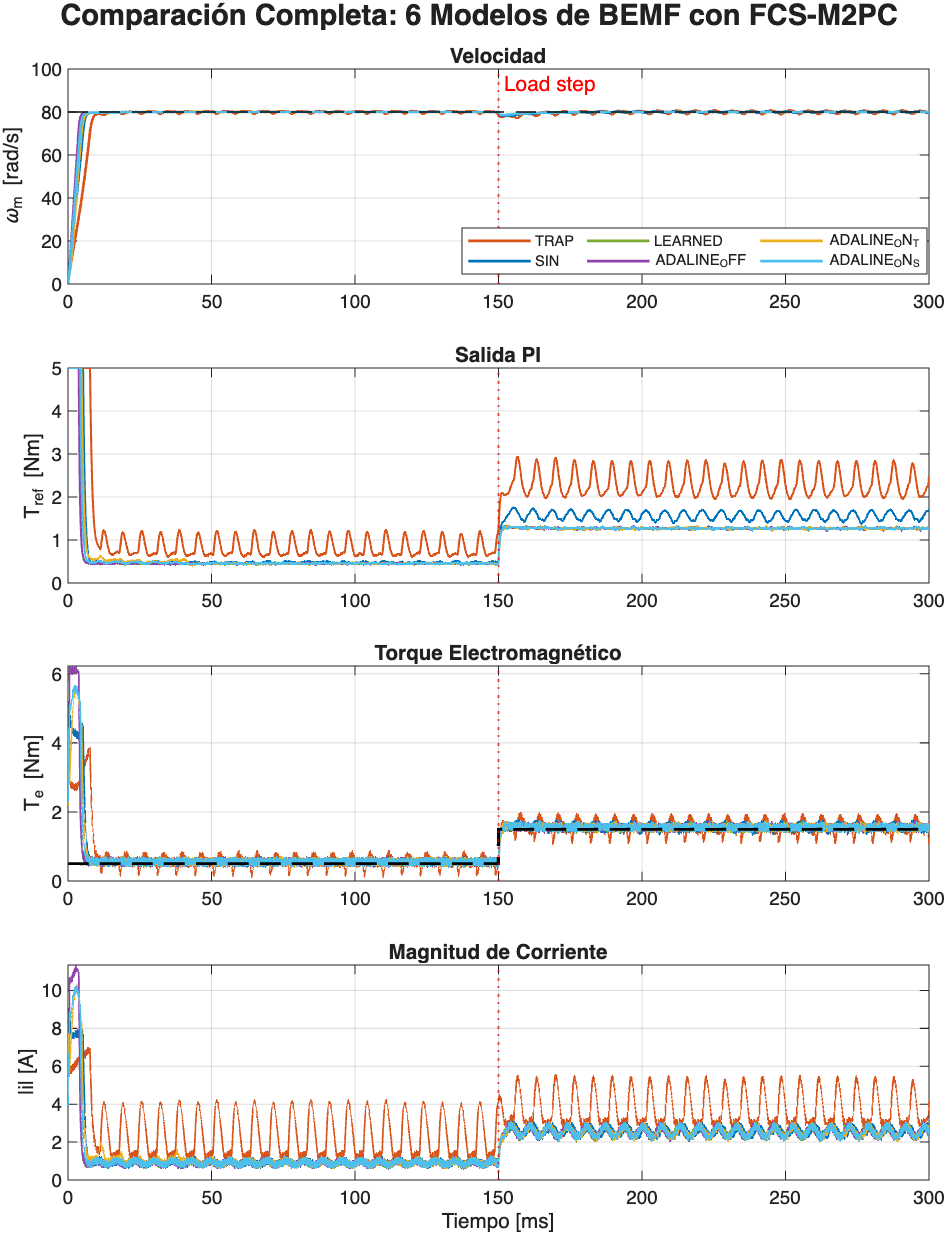
\includegraphics[width=0.35\linewidth]{fig/matlab_panorama.png}\\
        {\footnotesize FCS-M2PC con 6 BEMF y vs Load step}
      \end{center}
\end{frame}

% --- Slide 17: Figuras de simulación ---
\begin{frame}{Respuesta Temporal: Torque y Velocidad}
        \begin{center}
        \centering
        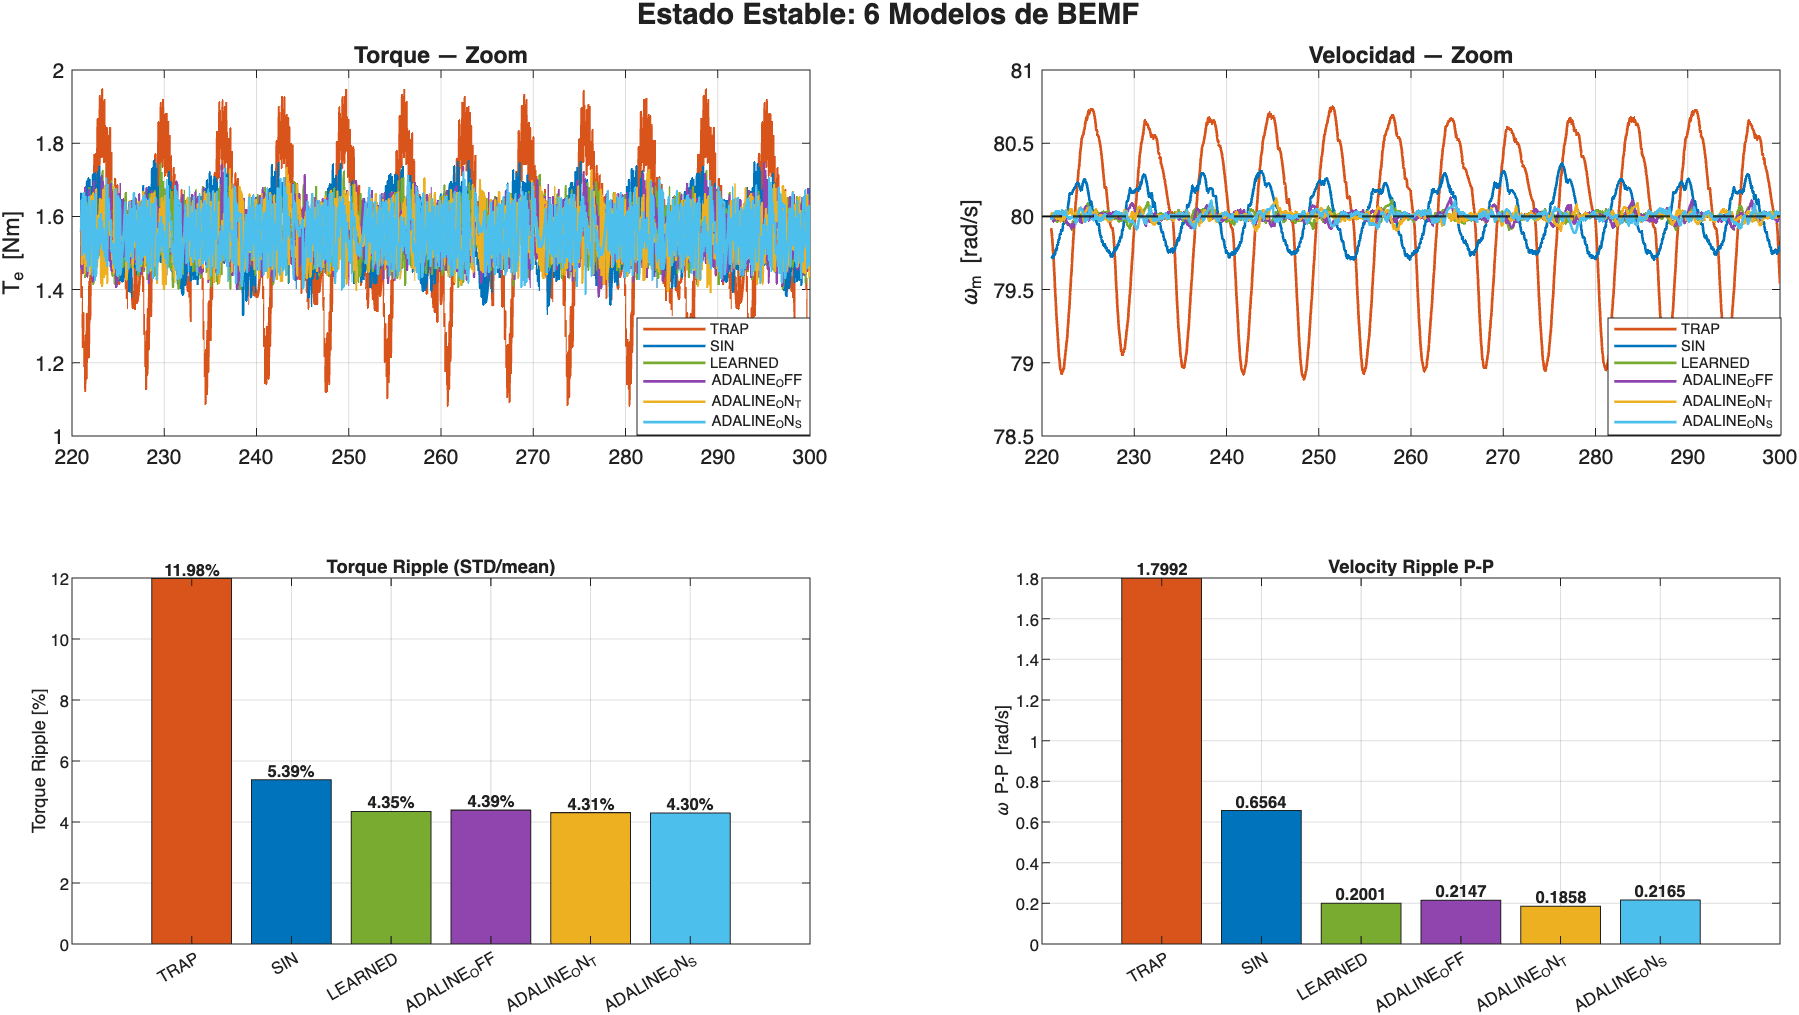
\includegraphics[width=0.75\linewidth]{fig/matlab_zoom_bars.png}\\
        {\footnotesize Zoom SS y Barras ripple}
        \end{center}
        

\end{frame}

% --- Slide 18: Convergencia ---
\begin{frame}{Convergencia del ADALINE Online}
    \begin{center}
        \centering
        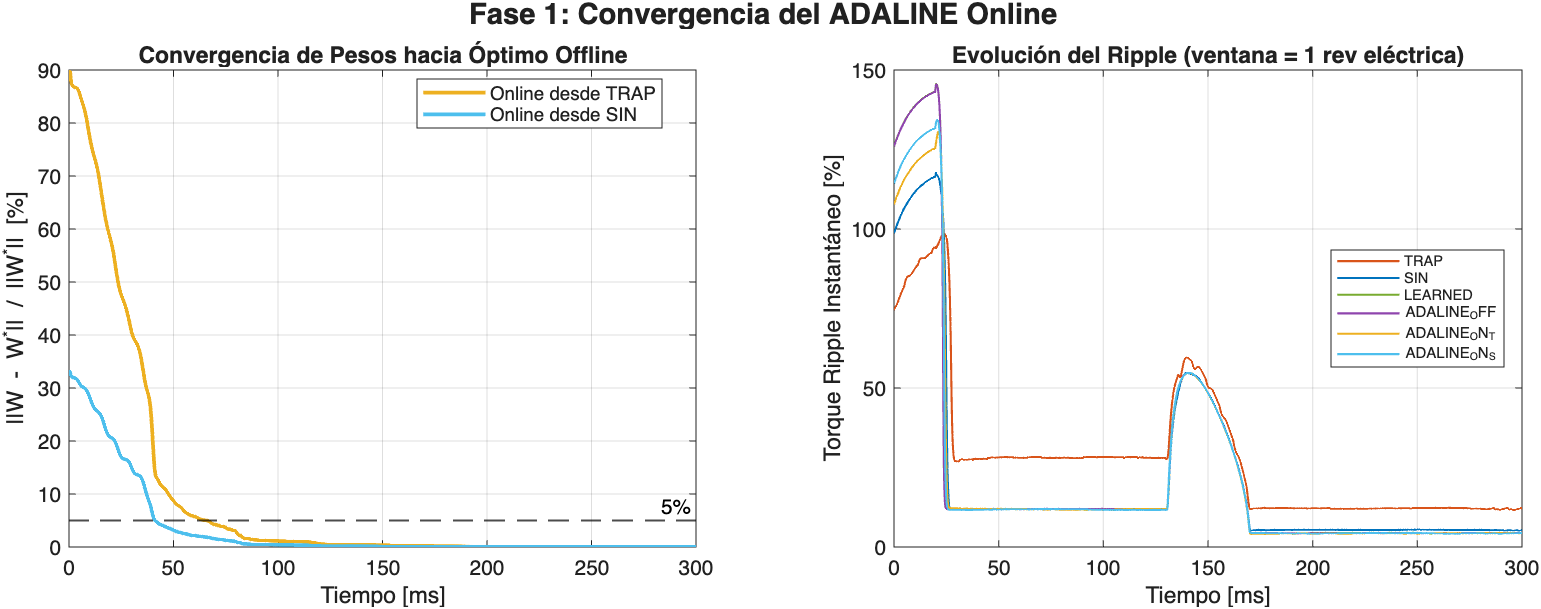
\includegraphics[width=0.95\linewidth]{fig/convergence_matlab.png}
        {\footnotesize Coeficientes de fourier por armónico}
      \end{center}
\end{frame}

%----------------- section 5 --------------------
\section{Trabajo Futuro: Control Repetitivo}
% ==============================================================
% SECCIÓN 5: TRABAJO FUTURO — CONTROL REPETITIVO
% ==============================================================

% --- Slide 18: Análisis a baja velocidad ---
\begin{frame}{Extensión: Análisis de Límites a Baja Velocidad}
    \textbf{Problema identificado:} el observador de BEMF falla cuando $\omega \rightarrow 0$,
    ya que $\mathbf{e} = K_e\,\omega\,\mathbf{s}(\theta) \rightarrow \mathbf{0}$ y la señal se
    hunde en el ruido del ADC ($\sigma \approx 50\,\text{mA}$, 12-bit).

    \vspace{0.2cm}

    \begin{columns}[T]
    \begin{column}{0.52\textwidth}
        \textbf{Se caracterizó en simulación:}
        \begin{itemize}
            \item Resolución del encoder vs.\ velocidad: por debajo de $\sim\!15$ rpm el encoder
                  queda ``congelado'' entre muestras $\rightarrow$ el observador debe interpolar.
            \item Ripple baseline del M2PC a \{5, 10, 20, 60\} rpm con encoder ideal
                  (velocidad impuesta, sin PI).
        \end{itemize}
        \vspace{0.2cm}
        \textbf{Conclusión:} el rizo crece sustancialmente a baja velocidad $\rightarrow$
        motiva extender el controlador para este régimen.
    \end{column}
    \begin{column}{0.45\textwidth}
        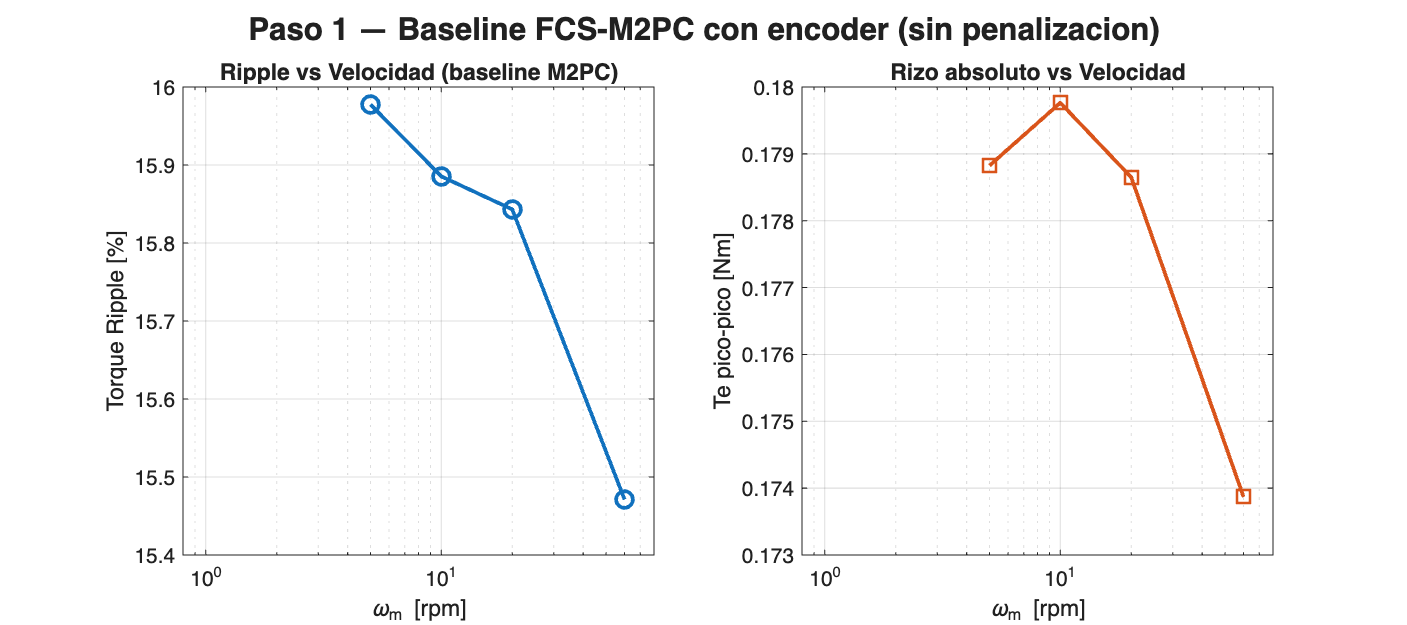
\includegraphics[width=\linewidth]{fig/baseline_ripple_vs_speed.png}
        {\tiny Ripple de par vs.\ velocidad — M2PC con encoder 2048\,PPR}
    \end{column}
    \end{columns}
\end{frame}

% --- Slide 19: Limitaciones actuales ---
\begin{frame}{¿Qué Falta? Fuentes de Rizo que ADALINE No Elimina}
    El ADALINE corrige el \textit{model mismatch} de BEMF, pero quedan fuentes de rizo \textbf{que no son error de BEMF}:
    
    \vspace{0.3cm}
    
    \begin{columns}[T]
    \begin{column}{0.48\textwidth}
        \begin{alertblock}{Fuentes residuales}
            \begin{itemize}
                \item \textbf{Cogging torque:} función de $\theta$, independiente de corriente. Armónicos 6to, 12vo.
                \item \textbf{Dead-time del inversor:} distorsiona el voltaje aplicado. Armónicos 5to/7mo.
                \item \textbf{Discretización M2PC:} $\rho$ finito $\rightarrow$ error de cuantización.
            \end{itemize}
        \end{alertblock}
    \end{column}
    \begin{column}{0.48\textwidth}
        \begin{exampleblock}{Propiedad común}
            Todas son \textbf{perturbaciones periódicas} con frecuencias múltiplos de la frecuencia eléctrica.
            
            \vspace{0.3cm}
            
            $\rightarrow$ Candidatas perfectas para \textbf{Control Repetitivo (RC)}.
        \end{exampleblock}
    \end{column}
    \end{columns}
\end{frame}

% --- Slide 19: Control Repetitivo ---
\begin{frame}{Control Repetitivo: Rechazo de Disturbios Periódicos}
    \textbf{Principio del Modelo Interno:} para rechazar una perturbación periódica de período $T$, el controlador debe contener el generador de señal periódica:
    \begin{equation}
        C_{RC}(z) = \frac{Q(z)\,z^{-N}}{1 - Q(z)\,z^{-N}} \cdot z^p \cdot G_f(z), \qquad N = T/T_s
    \end{equation}
    
    Esto provee \textbf{ganancia infinita en todos los armónicos} simultáneamente.
    
    \vspace{0.3cm}
    
    \begin{columns}[T]
    \begin{column}{0.48\textwidth}
        \textbf{Arquitectura propuesta:}
        \begin{enumerate}
            \item \textbf{ADALINE} (feedforward): corrige errores de BEMF $\rightarrow$ elimina rizo grueso.
            \item \textbf{RC} (feedback): compensa rizo residual periódico $\rightarrow$ elimina cogging, dead-time.
        \end{enumerate}
    \end{column}
    \begin{column}{0.48\textwidth}
        \textbf{Conexión ADALINE $\rightarrow$ RC:}
        \begin{itemize}
            \item Los pesos del ADALINE revelan el \textbf{espectro del motor}.
            \item Esto informa el diseño de $Q(z)$ y $G_f(z)$ del RC.
            \item Esquema RC selectivo: atacar solo los armónicos que ADALINE no puede eliminar.
        \end{itemize}
    \end{column}
    \end{columns}
\end{frame}

% --- Slide 20: Roadmap ---
\begin{frame}{Roadmap de la Investigación}
    \begin{center}
    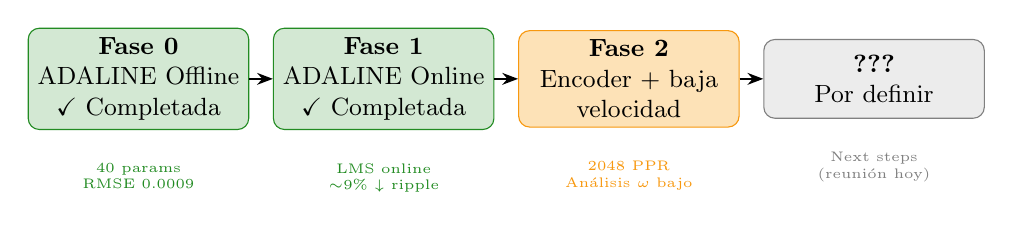
\begin{tikzpicture}[
        node distance=0.4cm and 0.3cm,
        phase/.style={draw, rounded corners, minimum width=2.8cm, minimum height=1cm, align=center, font=\small},
        done/.style={phase, fill=ForestGreen!20, draw=ForestGreen},
        curr/.style={phase, fill=YellowOrange!25, draw=YellowOrange},
        future/.style={phase, fill=gray!15, draw=gray},
        arrow/.style={-{Stealth[length=2mm]}, thick}
    ]
        \node[done] (f0) {\textbf{Fase 0}\\ADALINE Offline\\$\checkmark$ Completada};
        \node[done, right=of f0] (f1) {\textbf{Fase 1}\\ADALINE Online\\$\checkmark$ Completada};
        \node[curr, right=of f1] (f2) {\textbf{Fase 2}\\Encoder + baja\\velocidad};
        \node[future, right=of f2] (fq) {\textbf{???}\\Por definir};

        \draw[arrow] (f0) -- (f1);
        \draw[arrow] (f1) -- (f2);
        \draw[arrow] (f2) -- (fq);

        % Anotaciones debajo
        \node[below=0.3cm of f0, font=\tiny, align=center, text=ForestGreen] {40 params\\RMSE 0.0009};
        \node[below=0.3cm of f1, font=\tiny, align=center, text=ForestGreen] {LMS online\\$\sim$9\% $\downarrow$ ripple};
        \node[below=0.3cm of f2, font=\tiny, align=center, text=YellowOrange] {2048 PPR\\Análisis $\omega$ bajo};
        \node[below=0.3cm of fq, font=\tiny, align=center, text=gray] {Next steps\\(reunión hoy)};
    \end{tikzpicture}
    \end{center}
    
    \vspace{0.5cm}
    
    \textbf{Contribución principal:} Arquitectura en tres capas (ADALINE offline $\rightarrow$ ADALINE online $\rightarrow$ RC) que ataca el rizo de par desde la causa (BEMF) hasta el efecto residual (perturbaciones periódicas), con complejidad computacional compatible con DSP en tiempo real.
\end{frame}

% --- Slide 21: Conclusiones ---
\begin{frame}{Conclusiones Parciales}
    \begin{enumerate}
        \item El \textbf{ADALINE con base de Fourier} iguala la precisión de una NN profunda ($\sim$25k params) con solo \textbf{40 parámetros}, entrenado en \textbf{12 ms} vs.\ 30 s.
        
        \vspace{0.2cm}
        
        \item El \textbf{ADALINE online (LMS)} converge en $<$2 revoluciones eléctricas y alcanza el mismo rendimiento que el entrenamiento offline, demostrando capacidad de \textbf{auto-calibración}.
        
        \vspace{0.2cm}
        
        \item La integración ADALINE + FCS-M2PC reduce el rizo de par en $\sim$\textbf{9\%} respecto al modelo trapezoidal convencional, sin requerir datos previos del motor.
        
        \vspace{0.2cm}
        
        \item Los coeficientes de Fourier del ADALINE proveen una \textbf{representación interpretable} del motor que sirve como puente natural hacia el \textbf{Control Repetitivo}.
    \end{enumerate}
    
    \vspace{0.3cm}
    
    \begin{center}
        \textbf{Siguiente paso:} Integrar RC plug-in para atacar cogging torque y dead-time --- las fuentes de rizo que el ADALINE no puede eliminar por diseño.
    \end{center}
\end{frame}

%----------------------------------------------------------------------------------------
\begin{frame}{Referencias}
    \footnotesize
    \bibliographystyle{apalike}
    \bibliography{reference}
\end{frame}

\end{document}